

% Gradient Info
  
\tikzset {_n3q0y5w30/.code = {\pgfsetadditionalshadetransform{ \pgftransformshift{\pgfpoint{0 bp } { 0 bp }  }  \pgftransformrotate{0 }  \pgftransformscale{2 }  }}}
\pgfdeclarehorizontalshading{_3az8jupjp}{150bp}{rgb(0bp)=(0.94,0.98,1);
rgb(37.5bp)=(0.94,0.98,1);
rgb(55.77827453613281bp)=(0.8,0.92,1);
rgb(62.5bp)=(0.63,0.86,1);
rgb(100bp)=(0.63,0.86,1)}
\tikzset{every picture/.style={line width=0.75pt}} %set default line width to 0.75pt        

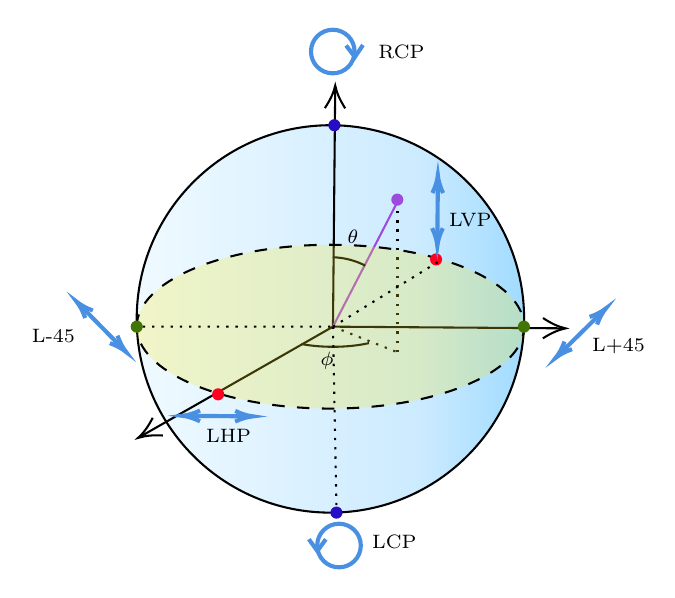
\begin{tikzpicture}[x=0.75pt,y=0.75pt,yscale=-1,xscale=1]
%uncomment if require: \path (0,300); %set diagram left start at 0, and has height of 300

%Shape: Circle [id:dp6406212717207735] 
\path  [shading=_3az8jupjp,_n3q0y5w30] (167.03,173.32) .. controls (167.03,121.78) and (208.82,80) .. (260.36,80) .. controls (311.9,80) and (353.68,121.78) .. (353.68,173.32) .. controls (353.68,224.87) and (311.9,266.65) .. (260.36,266.65) .. controls (208.82,266.65) and (167.03,224.87) .. (167.03,173.32) -- cycle ; % for fading 
 \draw   (167.03,173.32) .. controls (167.03,121.78) and (208.82,80) .. (260.36,80) .. controls (311.9,80) and (353.68,121.78) .. (353.68,173.32) .. controls (353.68,224.87) and (311.9,266.65) .. (260.36,266.65) .. controls (208.82,266.65) and (167.03,224.87) .. (167.03,173.32) -- cycle ; % for border 

%Straight Lines [id:da5120708694986456] 
\draw    (261.59,177.05) -- (169.42,229.66) ;
\draw [shift={(167.68,230.65)}, rotate = 330.28] [color={rgb, 255:red, 0; green, 0; blue, 0 }  ][line width=0.75]    (10.93,-4.9) .. controls (6.95,-2.3) and (3.31,-0.67) .. (0,0) .. controls (3.31,0.67) and (6.95,2.3) .. (10.93,4.9)   ;
%Straight Lines [id:da15371539088200992] 
\draw    (261.59,177.05) -- (262.66,62.87) ;
\draw [shift={(262.68,60.87)}, rotate = 90.54] [color={rgb, 255:red, 0; green, 0; blue, 0 }  ][line width=0.75]    (10.93,-4.9) .. controls (6.95,-2.3) and (3.31,-0.67) .. (0,0) .. controls (3.31,0.67) and (6.95,2.3) .. (10.93,4.9)   ;
%Straight Lines [id:da4675002401704563] 
\draw    (261.59,177.05) -- (371.68,177.85) ;
\draw [shift={(373.68,177.87)}, rotate = 180.42] [color={rgb, 255:red, 0; green, 0; blue, 0 }  ][line width=0.75]    (10.93,-4.9) .. controls (6.95,-2.3) and (3.31,-0.67) .. (0,0) .. controls (3.31,0.67) and (6.95,2.3) .. (10.93,4.9)   ;
%Straight Lines [id:da08410473848441524] 
\draw [color={rgb, 255:red, 157; green, 75; blue, 220 }  ,draw opacity=1 ]   (261.59,177.05) -- (292.68,116.85) ;
%Shape: Arc [id:dp875155371210051] 
\draw  [draw opacity=0] (261.48,143.6) .. controls (267.11,143.77) and (272.42,145.21) .. (277.14,147.63) -- (260.36,180.32) -- cycle ; \draw   (261.48,143.6) .. controls (267.11,143.77) and (272.42,145.21) .. (277.14,147.63) ;  
%Shape: Arc [id:dp8442710357943789] 
\draw  [draw opacity=0] (278.92,184.97) .. controls (274.03,186.09) and (268.05,186.75) .. (261.59,186.75) .. controls (256.04,186.75) and (250.84,186.26) .. (246.38,185.41) -- (261.59,177.05) -- cycle ; \draw   (278.92,184.97) .. controls (274.03,186.09) and (268.05,186.75) .. (261.59,186.75) .. controls (256.04,186.75) and (250.84,186.26) .. (246.38,185.41) ;  
%Straight Lines [id:da31008563400391076] 
\draw  [dash pattern={on 0.84pt off 2.51pt}]  (292.68,189.4) -- (292.68,116.85) ;
%Straight Lines [id:da7200714208810066] 
\draw  [dash pattern={on 0.84pt off 2.51pt}]  (261.59,177.05) -- (292.68,189.4) ;
%Shape: Ellipse [id:dp06773549043615945] 
\draw  [fill={rgb, 255:red, 248; green, 231; blue, 28 }  ,fill opacity=0.24 ][dash pattern={on 4.5pt off 4.5pt}] (167.03,177.06) .. controls (167.03,155.27) and (208.82,137.6) .. (260.36,137.6) .. controls (311.9,137.6) and (353.68,155.27) .. (353.68,177.06) .. controls (353.68,198.85) and (311.9,216.52) .. (260.36,216.52) .. controls (208.82,216.52) and (167.03,198.85) .. (167.03,177.06) -- cycle ;
%Shape: Ellipse [id:dp24576205607243373] 
\draw  [draw opacity=0][fill={rgb, 255:red, 38; green, 12; blue, 197 }  ,fill opacity=1 ][dash pattern={on 4.5pt off 4.5pt}] (259.36,80) .. controls (259.36,78.39) and (260.66,77.08) .. (262.26,77.08) .. controls (263.87,77.08) and (265.17,78.39) .. (265.17,80) .. controls (265.17,81.61) and (263.87,82.92) .. (262.26,82.92) .. controls (260.66,82.92) and (259.36,81.61) .. (259.36,80) -- cycle ;
%Shape: Ellipse [id:dp6984956246077939] 
\draw  [draw opacity=0][fill={rgb, 255:red, 38; green, 12; blue, 197 }  ,fill opacity=1 ][dash pattern={on 4.5pt off 4.5pt}] (260.36,266.65) .. controls (260.36,265.04) and (261.66,263.73) .. (263.26,263.73) .. controls (264.87,263.73) and (266.17,265.04) .. (266.17,266.65) .. controls (266.17,268.26) and (264.87,269.57) .. (263.26,269.57) .. controls (261.66,269.57) and (260.36,268.26) .. (260.36,266.65) -- cycle ;
%Shape: Ellipse [id:dp9059789894751615] 
\draw  [draw opacity=0][fill={rgb, 255:red, 255; green, 0; blue, 33 }  ,fill opacity=1 ][dash pattern={on 4.5pt off 4.5pt}] (203.36,209.65) .. controls (203.36,208.04) and (204.66,206.73) .. (206.26,206.73) .. controls (207.87,206.73) and (209.17,208.04) .. (209.17,209.65) .. controls (209.17,211.26) and (207.87,212.57) .. (206.26,212.57) .. controls (204.66,212.57) and (203.36,211.26) .. (203.36,209.65) -- cycle ;
%Shape: Ellipse [id:dp20089683016381765] 
\draw  [draw opacity=0][fill={rgb, 255:red, 255; green, 0; blue, 33 }  ,fill opacity=1 ][dash pattern={on 4.5pt off 4.5pt}] (308.36,144.65) .. controls (308.36,143.04) and (309.66,141.73) .. (311.26,141.73) .. controls (312.87,141.73) and (314.17,143.04) .. (314.17,144.65) .. controls (314.17,146.26) and (312.87,147.57) .. (311.26,147.57) .. controls (309.66,147.57) and (308.36,146.26) .. (308.36,144.65) -- cycle ;
%Shape: Ellipse [id:dp8254418229832045] 
\draw  [draw opacity=0][fill={rgb, 255:red, 65; green, 117; blue, 5 }  ,fill opacity=1 ][dash pattern={on 4.5pt off 4.5pt}] (350.68,177.06) .. controls (350.68,175.45) and (351.98,174.14) .. (353.59,174.14) .. controls (355.19,174.14) and (356.5,175.45) .. (356.5,177.06) .. controls (356.5,178.67) and (355.19,179.98) .. (353.59,179.98) .. controls (351.98,179.98) and (350.68,178.67) .. (350.68,177.06) -- cycle ;
%Shape: Ellipse [id:dp36388662554978257] 
\draw  [draw opacity=0][fill={rgb, 255:red, 65; green, 117; blue, 5 }  ,fill opacity=1 ][dash pattern={on 4.5pt off 4.5pt}] (164.13,177.06) .. controls (164.13,175.45) and (165.43,174.14) .. (167.03,174.14) .. controls (168.64,174.14) and (169.94,175.45) .. (169.94,177.06) .. controls (169.94,178.67) and (168.64,179.98) .. (167.03,179.98) .. controls (165.43,179.98) and (164.13,178.67) .. (164.13,177.06) -- cycle ;
%Shape: Ellipse [id:dp43839158045072046] 
\draw  [draw opacity=0][fill={rgb, 255:red, 157; green, 75; blue, 220 }  ,fill opacity=1 ][dash pattern={on 4.5pt off 4.5pt}] (289.68,115.85) .. controls (289.68,114.24) and (290.98,112.93) .. (292.59,112.93) .. controls (294.19,112.93) and (295.5,114.24) .. (295.5,115.85) .. controls (295.5,117.46) and (294.19,118.77) .. (292.59,118.77) .. controls (290.98,118.77) and (289.68,117.46) .. (289.68,115.85) -- cycle ;
%Straight Lines [id:da8188010633140681] 
\draw  [dash pattern={on 0.84pt off 2.51pt}]  (261.59,177.05) -- (314.17,144.65) ;
%Straight Lines [id:da4970670972010699] 
\draw  [dash pattern={on 0.84pt off 2.51pt}]  (169.94,177.06) -- (261.59,177.05) ;
%Shape: Circle [id:dp7168582977318296] 
\draw  [color={rgb, 255:red, 74; green, 144; blue, 226 }  ,draw opacity=1 ][line width=1.5]  (251,44.5) .. controls (251,38.7) and (255.7,34) .. (261.5,34) .. controls (267.3,34) and (272,38.7) .. (272,44.5) .. controls (272,50.3) and (267.3,55) .. (261.5,55) .. controls (255.7,55) and (251,50.3) .. (251,44.5) -- cycle ;
%Straight Lines [id:da42356120410196907] 
\draw  [dash pattern={on 0.84pt off 2.51pt}]  (261.59,177.05) -- (263.26,263.73) ;
%Shape: Circle [id:dp7373946176406471] 
\draw  [color={rgb, 255:red, 74; green, 144; blue, 226 }  ,draw opacity=1 ][line width=1.5]  (254,282.5) .. controls (254,276.7) and (258.7,272) .. (264.5,272) .. controls (270.3,272) and (275,276.7) .. (275,282.5) .. controls (275,288.3) and (270.3,293) .. (264.5,293) .. controls (258.7,293) and (254,288.3) .. (254,282.5) -- cycle ;
\draw  [color={rgb, 255:red, 74; green, 144; blue, 226 }  ,draw opacity=1 ][line width=1.5]  (276.05,41.35) -- (272.15,47.11) -- (267.91,41.59) ;
\draw  [color={rgb, 255:red, 74; green, 144; blue, 226 }  ,draw opacity=1 ][line width=1.5]  (258.14,279.47) -- (254.06,285.11) -- (249.99,279.47) ;
%Straight Lines [id:da31433845457985843] 
\draw [color={rgb, 255:red, 74; green, 144; blue, 226 }  ,draw opacity=1 ][line width=1.5]    (192,220.02) -- (220,220.24) ;
\draw [shift={(223,220.27)}, rotate = 180.45] [color={rgb, 255:red, 74; green, 144; blue, 226 }  ,draw opacity=1 ][line width=1.5]    (8.53,-2.57) .. controls (5.42,-1.09) and (2.58,-0.23) .. (0,0) .. controls (2.58,0.23) and (5.42,1.09) .. (8.53,2.57)   ;
\draw [shift={(189,220)}, rotate = 0.45] [color={rgb, 255:red, 74; green, 144; blue, 226 }  ,draw opacity=1 ][line width=1.5]    (8.53,-2.57) .. controls (5.42,-1.09) and (2.58,-0.23) .. (0,0) .. controls (2.58,0.23) and (5.42,1.09) .. (8.53,2.57)   ;
%Shape: Boxed Line [id:dp7497697764799951] 
\draw [color={rgb, 255:red, 74; green, 144; blue, 226 }  ,draw opacity=1 ][line width=1.5]    (312.11,107.13) -- (311.89,135.13) ;
\draw [shift={(311.87,138.13)}, rotate = 270.45] [color={rgb, 255:red, 74; green, 144; blue, 226 }  ,draw opacity=1 ][line width=1.5]    (8.53,-2.57) .. controls (5.42,-1.09) and (2.58,-0.23) .. (0,0) .. controls (2.58,0.23) and (5.42,1.09) .. (8.53,2.57)   ;
\draw [shift={(312.13,104.13)}, rotate = 90.45] [color={rgb, 255:red, 74; green, 144; blue, 226 }  ,draw opacity=1 ][line width=1.5]    (8.53,-2.57) .. controls (5.42,-1.09) and (2.58,-0.23) .. (0,0) .. controls (2.58,0.23) and (5.42,1.09) .. (8.53,2.57)   ;
%Shape: Boxed Line [id:dp3615276405181248] 
\draw [color={rgb, 255:red, 74; green, 144; blue, 226 }  ,draw opacity=1 ][line width=1.5]    (390.98,170.31) -- (371.02,189.96) ;
\draw [shift={(368.88,192.06)}, rotate = 315.45] [color={rgb, 255:red, 74; green, 144; blue, 226 }  ,draw opacity=1 ][line width=1.5]    (8.53,-2.57) .. controls (5.42,-1.09) and (2.58,-0.23) .. (0,0) .. controls (2.58,0.23) and (5.42,1.09) .. (8.53,2.57)   ;
\draw [shift={(393.12,168.21)}, rotate = 135.45] [color={rgb, 255:red, 74; green, 144; blue, 226 }  ,draw opacity=1 ][line width=1.5]    (8.53,-2.57) .. controls (5.42,-1.09) and (2.58,-0.23) .. (0,0) .. controls (2.58,0.23) and (5.42,1.09) .. (8.53,2.57)   ;
%Shape: Boxed Line [id:dp25245506689184194] 
\draw [color={rgb, 255:red, 74; green, 144; blue, 226 }  ,draw opacity=1 ][line width=1.5]    (140.17,167.15) -- (159.83,187.12) ;
\draw [shift={(161.93,189.26)}, rotate = 225.45] [color={rgb, 255:red, 74; green, 144; blue, 226 }  ,draw opacity=1 ][line width=1.5]    (8.53,-2.57) .. controls (5.42,-1.09) and (2.58,-0.23) .. (0,0) .. controls (2.58,0.23) and (5.42,1.09) .. (8.53,2.57)   ;
\draw [shift={(138.07,165.01)}, rotate = 45.45] [color={rgb, 255:red, 74; green, 144; blue, 226 }  ,draw opacity=1 ][line width=1.5]    (8.53,-2.57) .. controls (5.42,-1.09) and (2.58,-0.23) .. (0,0) .. controls (2.58,0.23) and (5.42,1.09) .. (8.53,2.57)   ;

% Text Node
\draw (267,129) node [anchor=north west][inner sep=0.75pt]  [font=\scriptsize]  {$\theta $};
% Text Node
\draw (254,188) node [anchor=north west][inner sep=0.75pt]  [font=\scriptsize]  {$\phi $};
% Text Node
\draw (282,40) node [anchor=north west][inner sep=0.75pt]  [font=\scriptsize] [align=left] {RCP};
% Text Node
\draw (279,276) node [anchor=north west][inner sep=0.75pt]  [font=\scriptsize] [align=left] {LCP};
% Text Node
\draw (199,225) node [anchor=north west][inner sep=0.75pt]  [font=\scriptsize] [align=left] {LHP};
% Text Node
\draw (316,121) node [anchor=north west][inner sep=0.75pt]  [font=\scriptsize] [align=left] {LVP};
% Text Node
\draw (385,181) node [anchor=north west][inner sep=0.75pt]  [font=\scriptsize] [align=left] {L+45};
% Text Node
\draw (115,177) node [anchor=north west][inner sep=0.75pt]  [font=\scriptsize] [align=left] {L-45};


\end{tikzpicture}
